\documentclass[10pt,xcolor={dvipsnames}]{beamer}
\usepackage[utf8]{inputenc}
\usepackage{graphicx}

\usetheme{Copenhagen}
\usecolortheme{seagull}

\usepackage{media9}
% \usepackage{media9}%
\newcommand{\includemovie}[3]{%
\includemedia[%
width=#1,height=#2,%
activate=pagevisible,%
deactivate=pageclose,%
addresource=#3,%
flashvars={%
src=#3 % same path as in addresource!
&autoPlay=true % default: false; if =true, automatically starts playback after activation (see option ‘activation)’
&loop=true % if loop=true, media is played in a loop
&controlBarAutoHideTimeout=0 %  time span before auto-hide
}%
]{}{StrobeMediaPlayback.swf}%
}% end of the new command

\usepackage{booktabs,siunitx}
\usepackage{multirow}
\usepackage[flushleft]{threeparttable}


\usepackage{amsmath}
\usepackage{stmaryrd}

\usepackage{amssymb}% http://ctan.org/pkg/amssymb
\usepackage{pifont}% http://ctan.org/pkg/pifont

\usepackage{animate}
\usepackage{adjustbox}

\usepackage{tikz}
\usepackage{amsfonts}
\usepackage{xcolor}
\usepackage{biblatex}
\usepackage{hyperref}
\usetikzlibrary{shapes,
                tikzmark}
\tikzset{every tikzmarknode/.style={%
        draw=red, semithick, inner sep=2pt}
        % invisible/.style={opacity=0},
        % tikzmarknode/.style={opacity=1},
        % alt/.code args={<#1>#2#3}{%
        % \alt<#1>{\pgfkeysalso{#2}}{\pgfkeysalso{#3}} % \pgfkeysalso doesn't change the path
        % },
        }

\tiny\bibliography{references.bib}
\usetikzlibrary{calc}
\DeclareMathOperator*{\argmax}{arg\,max}
\DeclareMathOperator*{\argmin}{arg\,min}
\DeclareMathOperator*{\argminB}{argmin}

\definecolor{red}{rgb}{1.00,0.00,0.00}
\definecolor{blue}{rgb}{0.00,0.00,1.00}
\definecolor{dblue}{rgb}{0.00,0.00,0.40}
\definecolor{green}{rgb}{0.4,1.00,0.0}
\definecolor{dgreen}{rgb}{0.0,0.40,0.0}
\definecolor{yellow}{rgb}{0.5,0.5,0.0}

%\renewcommand<>{\item}[1]{\only#2{\beameroriginal{\item}{#1}}}


%%%%%%%%%%%%%%%%%%%%%%%%%%%%%%%%%%%%%%%%%%%%%%%%%%%%%%%%%%%%%%%%%%%%%%%%%%%%%%%%%%%%%%%%%%%%%%%%%%%%%%%%%%%%%%%%%%%%%%%%---
%This block of code defines the information to appear in the
%Title page
\title[]
{\large Meta-Reinforcement Learning and Causality for Multi-tasking in Robots with Redundant Kinematics}

\subtitle{1st Year Update}

\author[Joel Baptista] % (optional)
{Joel Baptista}

% \institute[VFU] % (optional)
% {
%   \inst{1}%
%   Institute of Electronics and Informatics Engineering of Aveiro\\
%   University of Aveiro, Portugal
%   \and
%   \inst{2}%
%   Department of Mechanical Engineering\\
%   University of Aveiro, Portugal
% }

\date[2024/04/11] % (optional)
{11/04/2024}

% \begin{block}{}
% % \cite{DAA}
% \end{block}

\titlegraphic{\begin{center}
\begin{tabular}{c}
%\includegraphics[height=1cm]{img/cytedlogo} &

\includegraphics[height=1cm]{img/Logo-UA-300x300} 
\end{tabular}
\end{center}
}

\setbeamertemplate{footline}[frame number]
\setbeamertemplate{navigation symbols}{}

%End of title page configuration block
%%%%%%%%%%%%%%%%%%%%%%%%%%%%%%%%%%%%%%%%%%%%%%%%%%%%%%%%%%%%%%%%%%%%%%%%%%%%%%%%%%%%%%%%%%%%%%%%%%%%%%%%%%%%%%%%%%%%%%%%---



%%%%%%%%%%%%%%%%%%%%%%%%%%%%%%%%%%%%%%%%%%%%%%%%%%%%%%%%%%%%%%%%%%%%%%%%%%%%%%%%%%%%%%%%%%%%%%%%%%%%%%%%%%%%%%%%%%%%%%%%---
%The next block of commands puts the table of contents at the 
%beginning of each section and highlights the current section:

\AtBeginSection[]
{
  \begin{frame}
    \frametitle{Table of Contents}
    \tableofcontents[currentsection]
  \end{frame}
}
%%%%%%%%%%%%%%%%%%%%%%%%%%%%%%%%%%%%%%%%%%%%%%%%%%%%%%%%%%%%%%%%%%%%%%%%%%%%%%%%%%%%%%%%%%%%%%%%%%%%%%%%%%%%%%%%%%%%%%%%---


\begin{document}

%The next statement creates the title page.
\frame{\titlepage}


%%%%%%%%%%%%%%%%%%%%%%%%%%%%%%%%%%%%%%%%%%%%%%%%%%%%%%%%%%%%%%%%%%%%%%%%%%%%%%%%%%%%%%%%%%%%%%%%%%%%%%%%%%%%%%%%%%%%%%%%
%This block of code is for the table of contents after
%the title page

%%%%%%%%%%%%%%%%%%%%%%%%%%%%%%%%%%%%%%%%%%%%%%%%%%%%%%%%%%%%%%%%%%%%%%%%%%%%%%%%%%%%%%%%%%%%%%%%%%%%%%%%%%%%%%%%%%%%%%%%

%%%%%%%%%%%%%%%%%%%%%%%%%%%%%%%%%%%%%%%%%%%%%%%%%%%%%%%%%%%%%%%%%%%%%%%%%%%%%%%%%%%%%%%%%%%%%%%%%%%%%%%%%%%%%%%%%%%%%%%%
\section{Introduction}
%%%%%%%%%%%%%%%%%%%%%%%%%%%%%%%%%%%%%%%%%%%%%%%%%%%%%%%%%%%%%%%%%%%%%%%%%%%%%%%%%%%%%%%%%%%%%%%%%%%%%%%%%%%%%%%%%%%%%%%%%
\subsection{Focus}
%%%%%%%%%%%%%%%%%%%%%%%%%%%%%%%%%%%%%%%%%%%%%%%%%%%%%%%%%%%%%%%%%%%%%%%%%%%%%%%%%%%%%%%%%%%%%%%%%%%%%%%%%%%%%%%%%%%%%%%%%

%%%%%%%%%%%%%%%%%%%%%%%%%%%%%%%%%%%%%%%%%%%%%%%%%%%%%%%%%%%%%%%%%%%%%%%%%%%%%%%%%%%%%%%%%%%%%%%%%%%%%%%%%%%%%%%%%%%%%%%%%
\begin{frame}{Focus}
  \begin{figure}
    \centering
    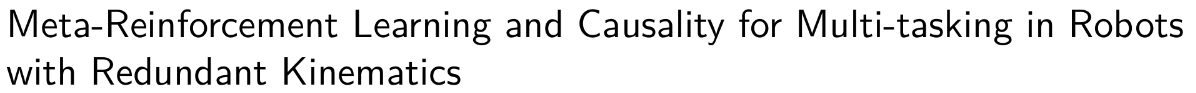
\includegraphics[width=\textwidth]{img/title.png}
  \end{figure}
  \pause
  Translation: Explore different learning methodologies to create intelligent agents that can control robots in difficult tasks
\end{frame}
%%%%%%%%%%%%%%%%%%%%%%%%%%%%%%%%%%%%%%%%%%%%%%%%%%%%%%%%%%%%%%%%%%%%%%%%%%%%%%%%%%%%%%%%%%%%%%%%%%%%%%%%%%%%%%%%%%%%%%%%
\begin{frame}{Focus}
  \begin{figure}
    \centering
    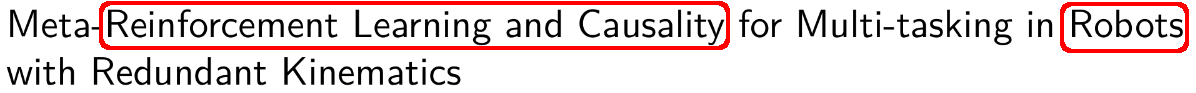
\includegraphics[width=\textwidth]{img/title_annotated.png}
  \end{figure}
  Translation: Explore different learning methodologies to create intelligent agents that can control robots in difficult tasks
\end{frame}
%%%%%%%%%%%%%%%%%%%%%%%%%%%%%%%%%%%%%%%%%%%%%%%%%%%%%%%%%%%%%%%%%%%%%%%%%%%%%%%%%%%%%%%%%%%%%%%%%%%%%%%%%%%%%%%%%%%%%%%%%
\subsection{Motivation}
%%%%%%%%%%%%%%%%%%%%%%%%%%%%%%%%%%%%%%%%%%%%%%%%%%%%%%%%%%%%%%%%%%%%%%%%%%%%%%%%%%%%%%%%%%%%%%%%%%%%%%%%%%%%%%%%%%%%%%%%%
\begin{frame}{Motivation}
  \begin{figure}
    \centering
    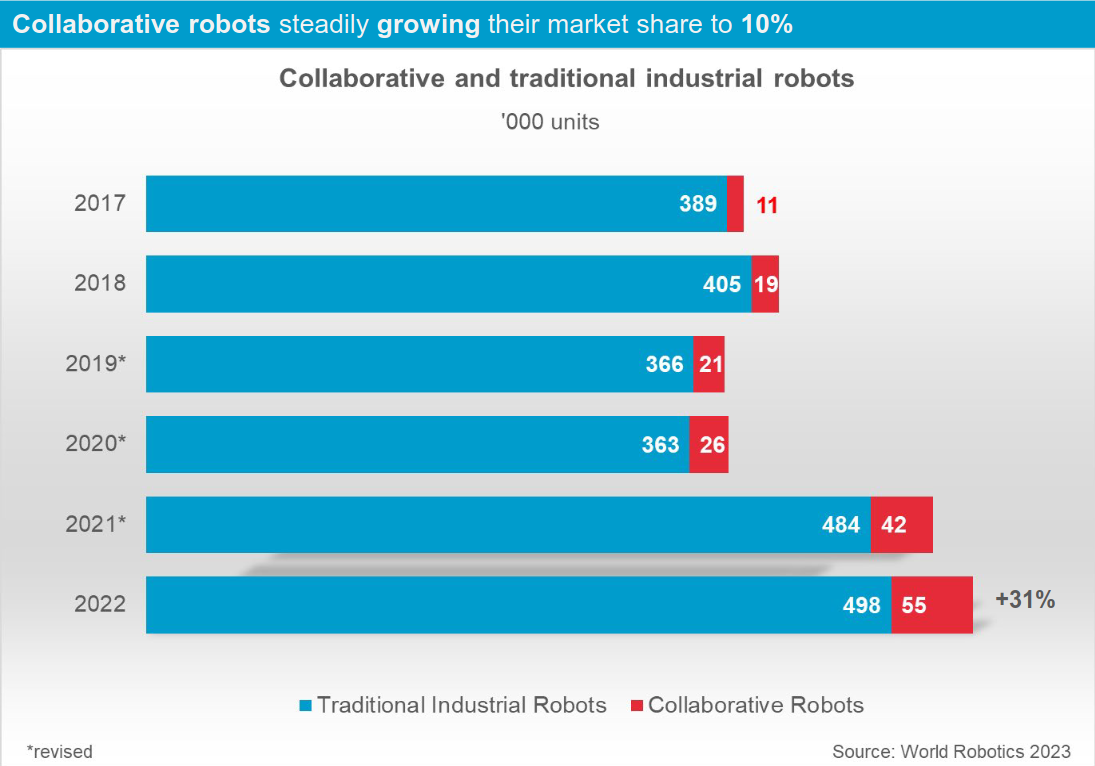
\includegraphics[width=0.7\textwidth]{img/cobot_hist.png}
    \caption{Collaborative and traditional industrial robots' growth\footnotemark}
  \end{figure}
  \footnotetext[1]{Source: \href{https://ifr.org/img/worldrobotics/2023_WR_extended_version.pdf}{World Robotics Report 2023 - Press Conference} }
\end{frame}
%%%%%%%%%%%%%%%%%%%%%%%%%%%%%%%%%%%%%%%%%%%%%%%%%%%%%%%%%%%%%%%%%%%%%%%%%%%%%%%%%%%%%%%%%%%%%%%%%%%%%%%%%%%%%%%%%%%%%%%%%
\begin{frame}{Motivation}
  \begin{figure}[ht]
    \begin{minipage}[b]{0.49\linewidth}
        \centering
        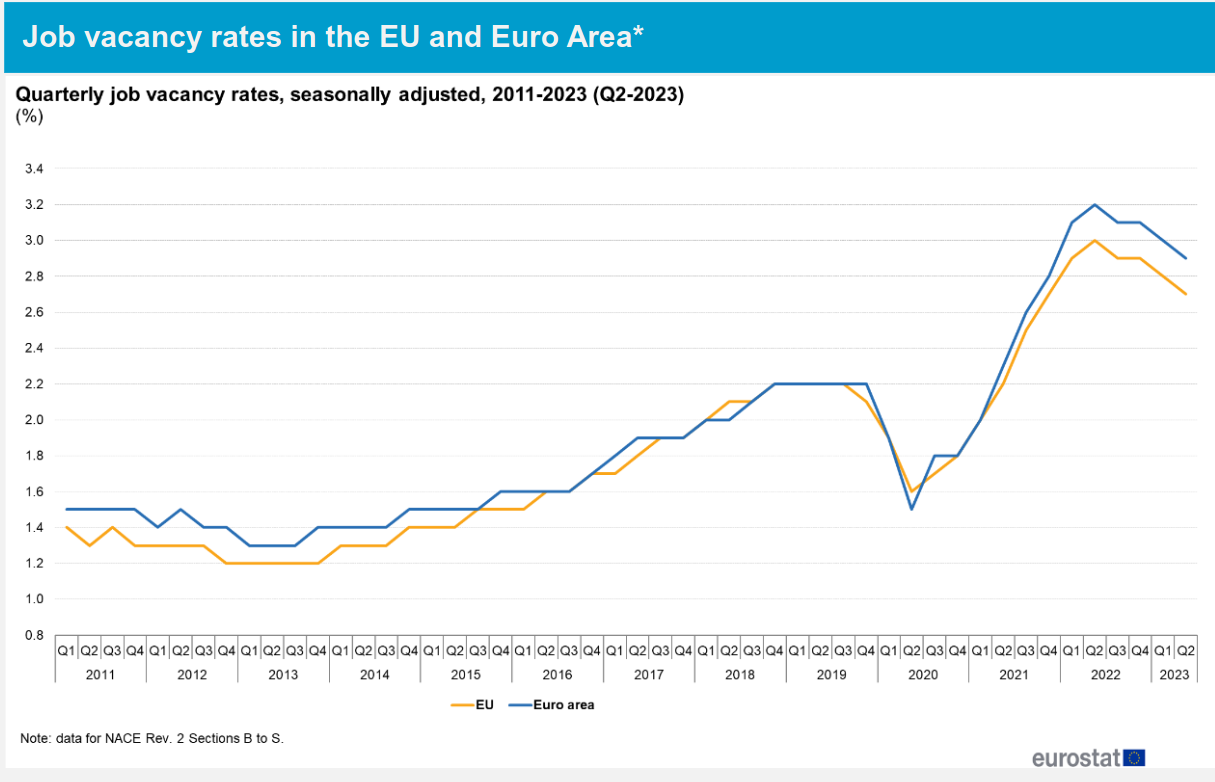
\includegraphics[width=\textwidth, height=0.7\textwidth]{img/job_vacancy.png}
    \end{minipage}
    \begin{minipage}[b]{0.49\linewidth}
        \centering
        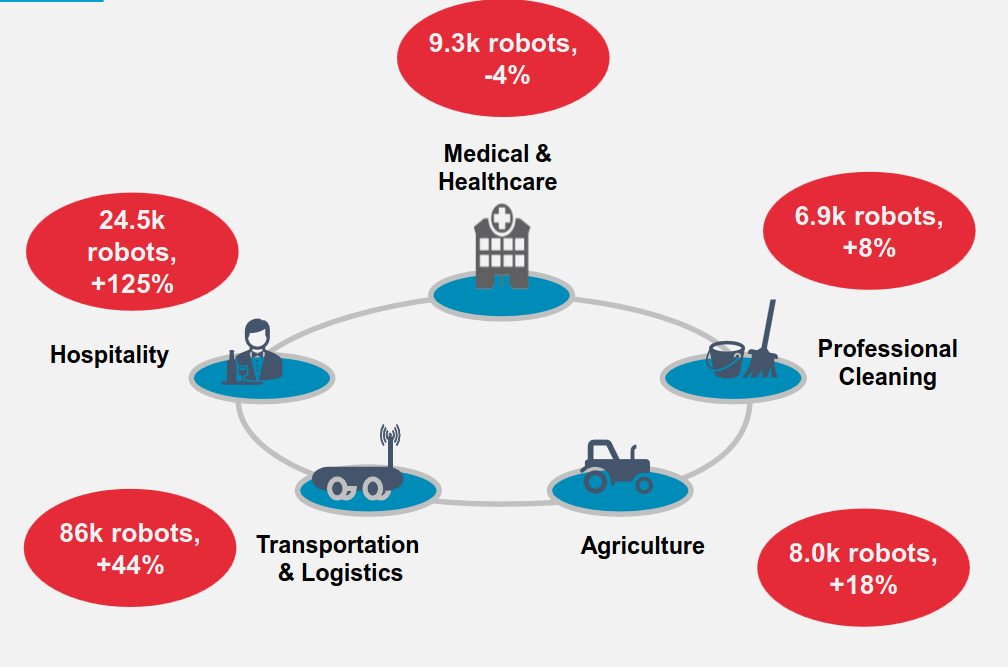
\includegraphics[width=\textwidth]{img/service_robots.png}
    \end{minipage}
    \caption{Job vacancy and service robots' growth\footnotemark[1]}
  \end{figure}
  Job vacancy is rising and the field of service robots is growing in response
  
  \footnotetext[1]{Source: \href{https://ifr.org/img/worldrobotics/2023_WR_extended_version.pdf}{World Robotics Report 2023 - Press Conference} }
\end{frame}
%%%%%%%%%%%%%%%%%%%%%%%%%%%%%%%%%%%%%%%%%%%%%%%%%%%%%%%%%%%%%%%%%%%%%%%%%%%%%%%%%%%%%%%%%%%%%%%%%%%%%%%%%%%%%%%%%%%%%%%%%
\begin{frame}{Motivation}
  Cobots and Service Robots interact in more complex and uncontrolled environments, ...

  \pause
  ... therefore, they need to be more \textbf{\underline{flexible and adaptable}} to different tasks.

\end{frame}
%%%%%%%%%%%%%%%%%%%%%%%%%%%%%%%%%%%%%%%%%%%%%%%%%%%%%%%%%%%%%%%%%%%%%%%%%%%%%%%%%%%%%%%%%%%%%%%%%%%%%%%%%%%%%%%%%%%%%%%%%

\section{Why Reinforcement Learning?}
%%%%%%%%%%%%%%%%%%%%%%%%%%%%%%%%%%%%%%%%%%%%%%%%%%%%%%%%%%%%%%%%%%%%%%%%%%%%%%%%%%%%%%%%%%%%%%%%%%%%%%%%%%%%%%%%%%%%%%%%%
\subsection{Reinforcement Learning}
%%%%%%%%%%%%%%%%%%%%%%%%%%%%%%%%%%%%%%%%%%%%%%%%%%%%%%%%%%%%%%%%%%%%%%%%%%%%%%%%%%%%%%%%%%%%%%%%%%%%%%%%%%%%%%%%%%%%%%%%%
\begin{frame}{Reinforcement Learning}
    \begin{figure}
      \centering
      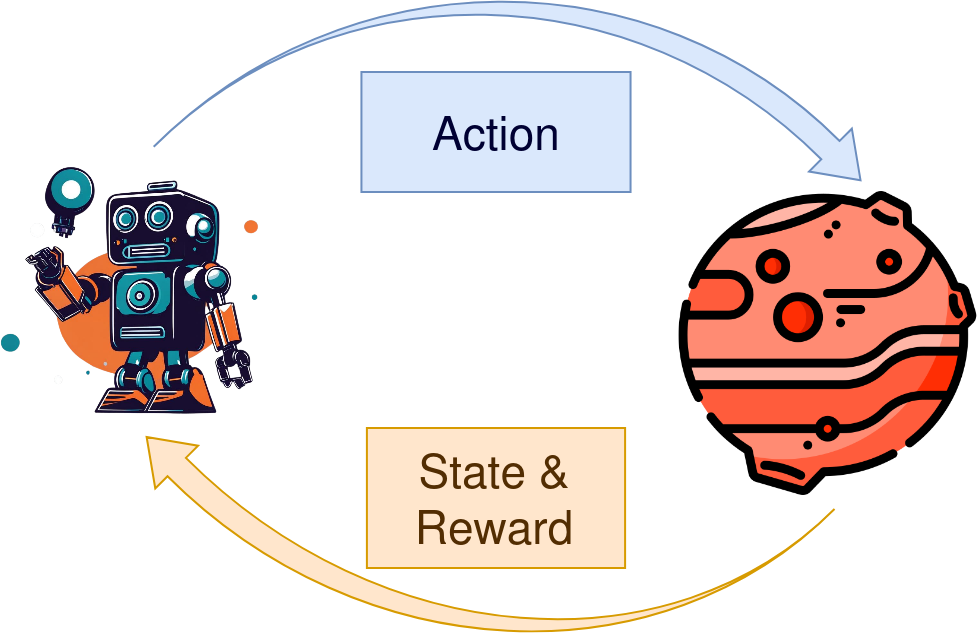
\includegraphics[width=0.6\textwidth]{img/rl-cycle.png}
    \end{figure}
    Learns to accomplish a goal by \textbf{\underline{interacting}} with an environment, receiving rewards and penalties.
\end{frame}

%%%%%%%%%%%%%%%%%%%%%%%%%%%%%%%%%%%%%%%%%%%%%%%%%%%%%%%%%%%%%%%%%%%%%%%%%%%%%%%%%%%%%%%%%%%%%%%%%%%%%%%%%%%%%%%%%%%%%%%%%
\subsection{Reinforcement Learning}
%%%%%%%%%%%%%%%%%%%%%%%%%%%%%%%%%%%%%%%%%%%%%%%%%%%%%%%%%%%%%%%%%%%%%%%%%%%%%%%%%%%%%%%%%%%%%%%%%%%%%%%%%%%%%%%%%%%%%%%%%

\begin{frame}{RL vs Traditional Control}
    \begin{figure}[ht]
        \begin{minipage}[b]{0.3\linewidth}
            \centering
            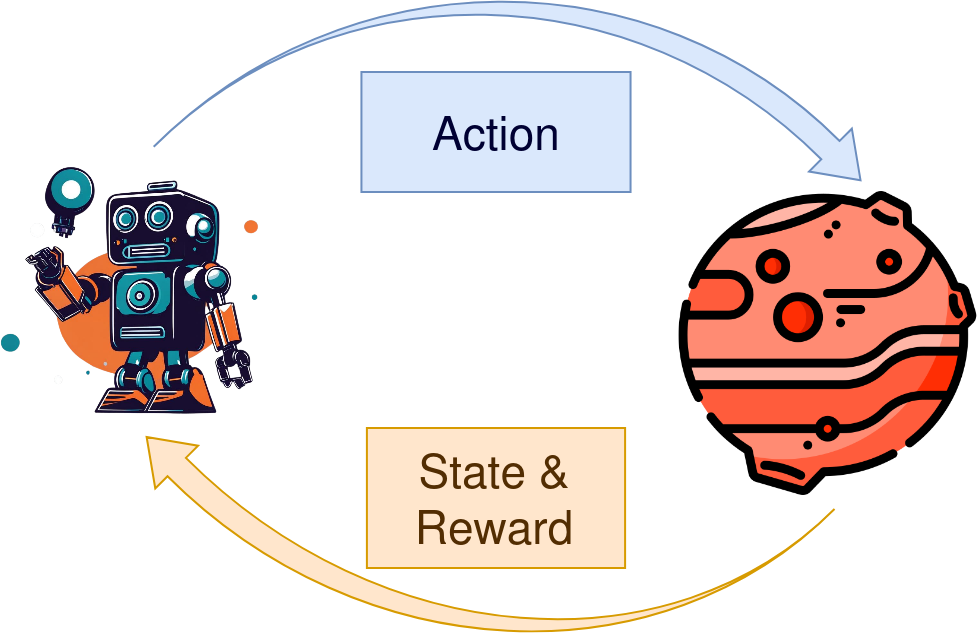
\includegraphics[width=\textwidth]{img/rl-cycle.png}
            \caption{\small Reinforcement Learning Cycle}
        \end{minipage}
        \begin{minipage}[b]{0.68\linewidth}
            \centering
            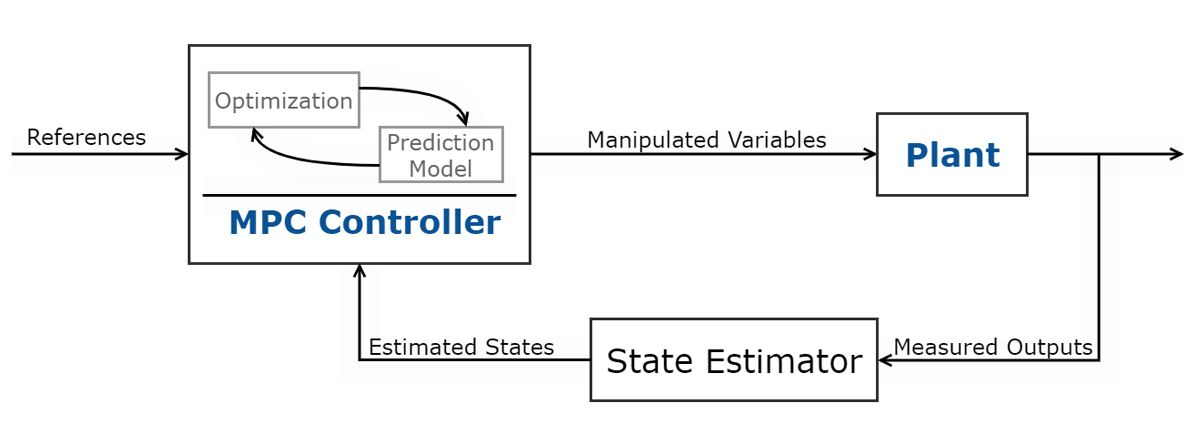
\includegraphics[width=\textwidth]{img/mpc.jpg}
            \caption{\small Model Predictive Control Cycle}
        \end{minipage}
    \end{figure}

    Just to mention that there are other methods to control robots, such as MDP, but they are not as flexible as RL.
\end{frame}

%%%%%%%%%%%%%%%%%%%%%%%%%%%%%%%%%%%%%%%%%%%%%%%%%%%%%%%%%%%%%%%%%%%%%%%%%%%%%%%%%%%%%%%%%%%%%%%%%%%%%%%%%%%%%%%%%%%%%%%%%
\begin{frame}{RL vs Traditional Control}

    \begin{center}
        \href{run:img/mpc-compressed.mp4}{
        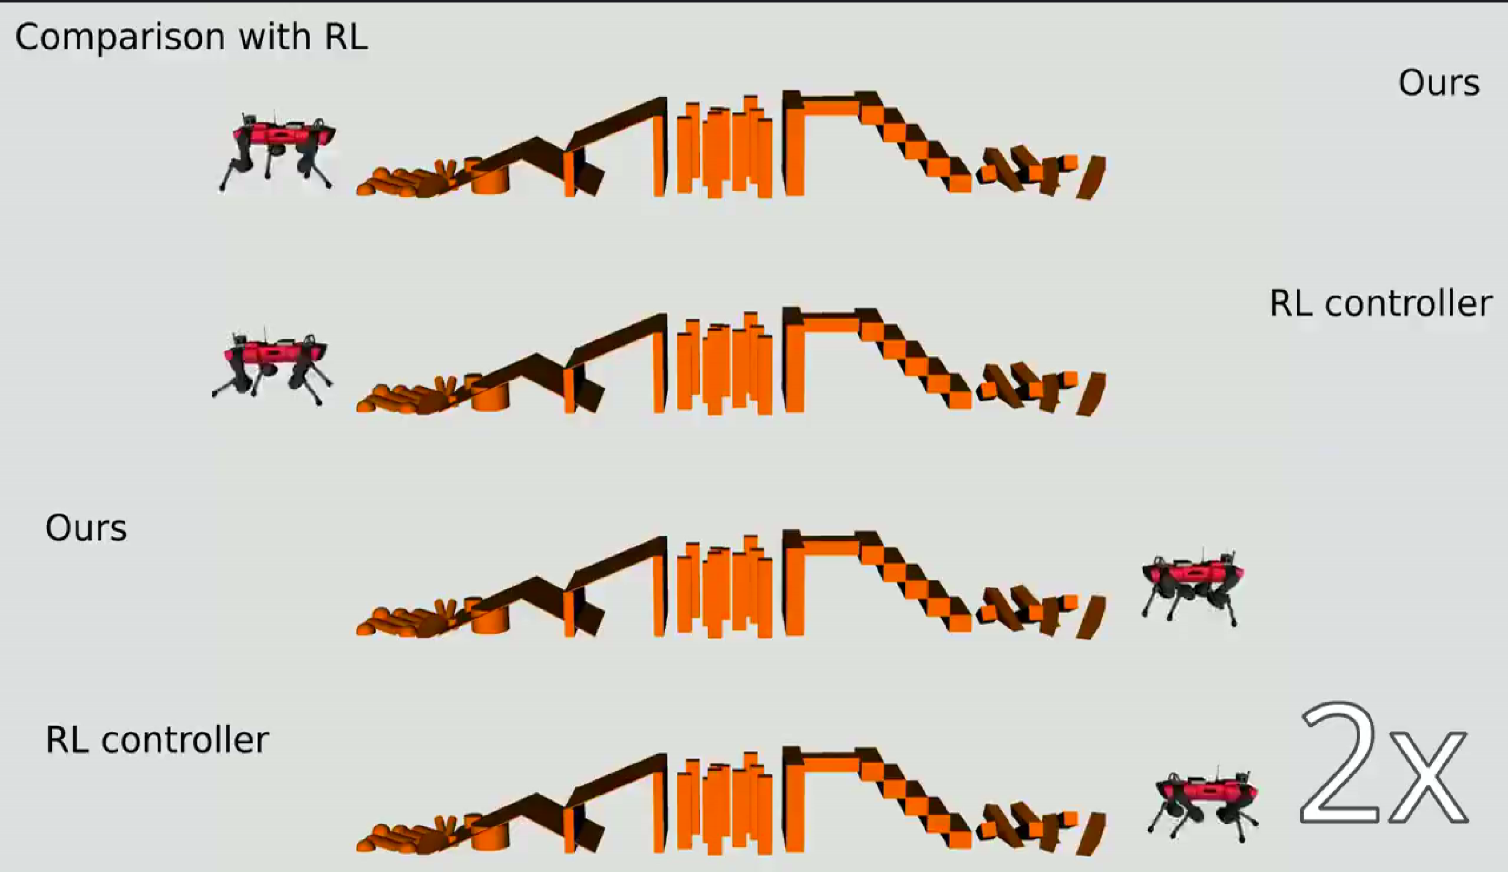
\includegraphics[scale=0.20]
        {img/mpc-thumb.png}
        }
    \end{center}
    \footnotetext[2]{Source: \href{https://www.youtube.com/watch?v=v6MhPl2ICsc}{Robotics Systems Lab: Legged Robotics at ETH Zurich}}

\end{frame}

%%%%%%%%%%%%%%%%%%%%%%%%%%%%%%%%%%%%%%%%%%%%%%%%%%%%%%%%%%%%%%%%%%%%%%%%%%%%%%%%%%%%%%%%%%%%%%%%%%%%%%%%%%%%%%%%%%%%%%%%%
\begin{frame}{RL vs Traditional Control}
    \begin{center}
        \href{run:img/fetch.mp4}{
        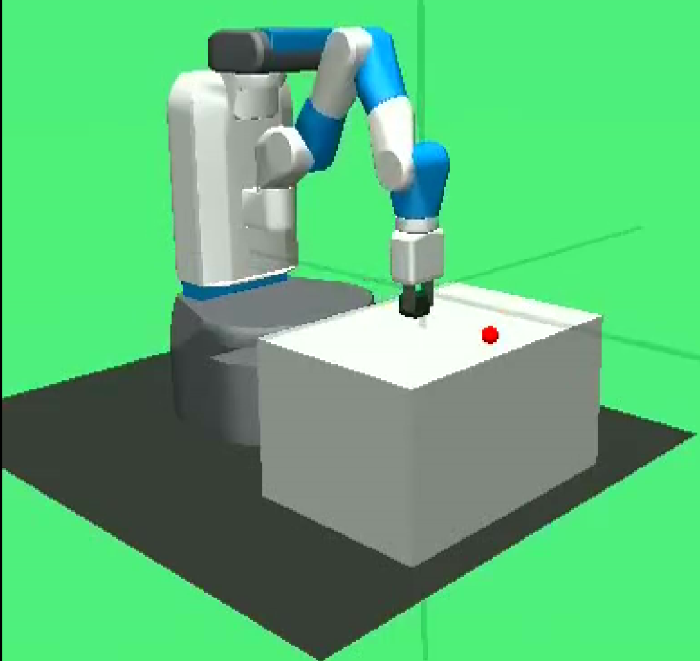
\includegraphics[scale=0.30]
        {img/fetch.png}
        }
    \end{center}
\end{frame}

\begin{frame}{RL vs Optimal Control}
    \begin{figure}
        \centering
        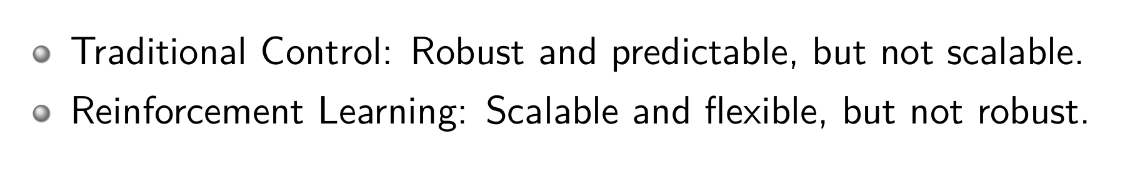
\includegraphics[width=\textwidth]{img/rl_vs_oc.png}
      \end{figure}
\end{frame}
\begin{frame}{RL vs Optimal Control}

    \begin{figure}
        \centering
        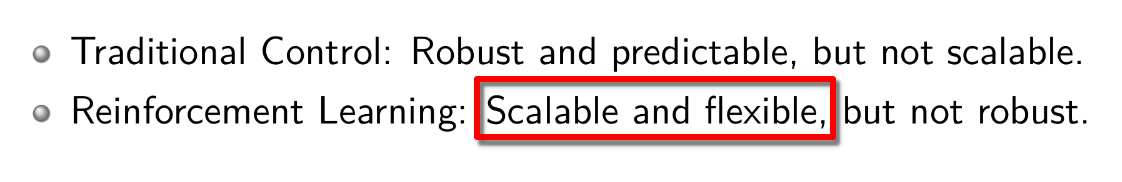
\includegraphics[width=\textwidth]{img/rl_vs_oc_annotated.png}
      \end{figure}
\end{frame}

\section{Why Causality?}
%%%%%%%%%%%%%%%%%%%%%%%%%%%%%%%%%%%%%%%%%%%%%%%%%%%%%%%%%%%%%%%%%%%%%%%%%%%%%%%%%%%%%%%%%%%%%%%%%%%%%%%%%%%%%%%%%%%%%%%%%
\subsection{Intuition}
%%%%%%%%%%%%%%%%%%%%%%%%%%%%%%%%%%%%%%%%%%%%%%%%%%%%%%%%%%%%%%%%%%%%%%%%%%%%%%%%%%%%%%%%%%%%%%%%%%%%%%%%%%%%%%%%%%%%%%%%%
\begin{frame}{Intuition}
    \begin{figure}
        \begin{minipage}[t]{0.30\linewidth}
            \centering
            \vspace{0pt}
            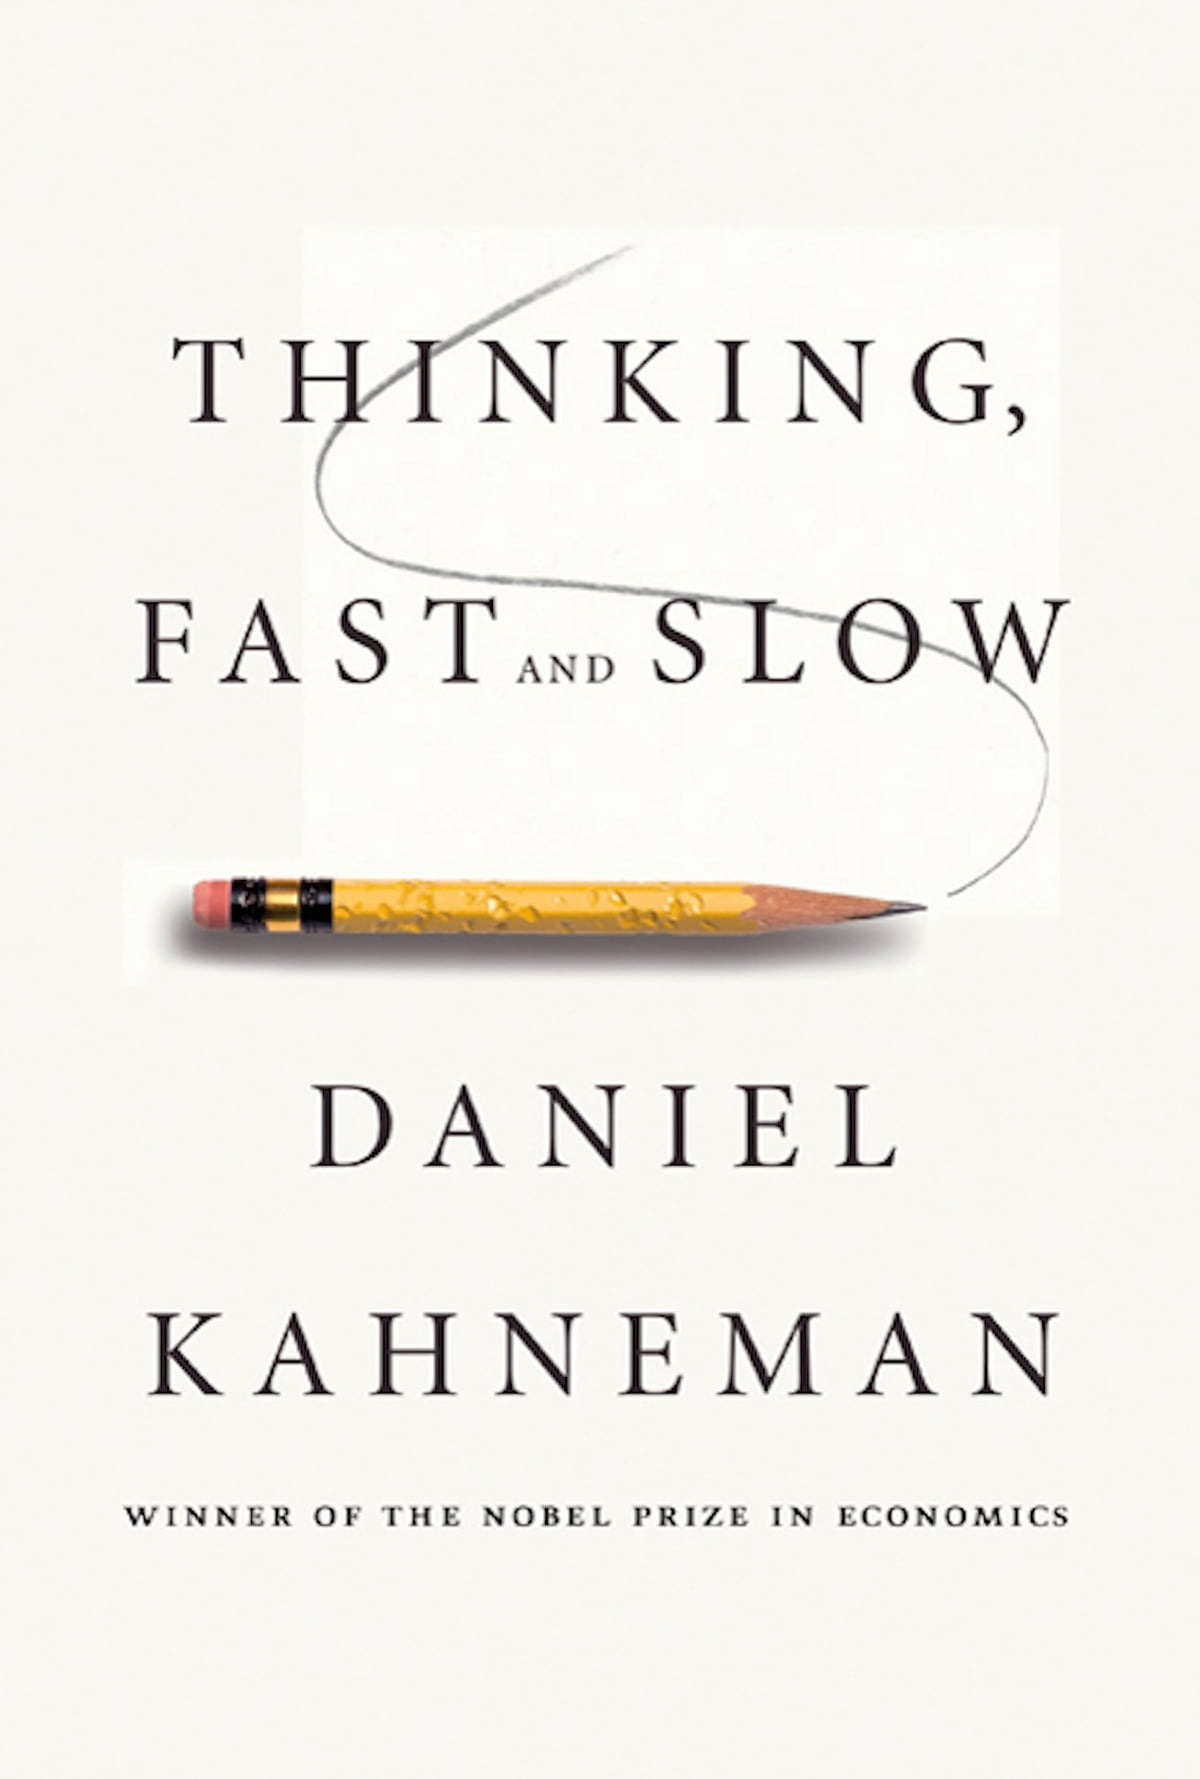
\includegraphics[width=\textwidth]{img/TFS.jpg}
        \end{minipage}
        \hspace{0.5cm}
        \begin{minipage}[t]{0.5\linewidth}
            \vspace{1cm}
            \begin{itemize}
                \item \textbf{Fast Thinking}: Correlation, pattern recognition, subconscious, ...
                \item \textbf{Slow Thinking}: Logical (causal), calculating, conscious, ...
            \end{itemize}
        \end{minipage}
    \end{figure}
    Many researchers believe that AI can only utilize "fast thinking" (System I). They propose causality to reach "slow thinking" (System II).
\end{frame}
%%%%%%%%%%%%%%%%%%%%%%%%%%%%%%%%%%%%%%%%%%%%%%%%%%%%%%%%%%%%%%%%%%%%%%%%%%%%%%%%%%%%%%%%%%%%%%%%%%%%%%%%%%%%%%%%%%%%%%%%%
\subsection{Correlation vs Causation}
%%%%%%%%%%%%%%%%%%%%%%%%%%%%%%%%%%%%%%%%%%%%%%%%%%%%%%%%%%%%%%%%%%%%%%%%%%%%%%%%%%%%%%%%%%%%%%%%%%%%%%%%%%%%%%%%%%%%%%%%%

\begin{frame}{Correlation vs Causation}
    \begin{figure}[t]
        \centering
        \vspace{0pt}
        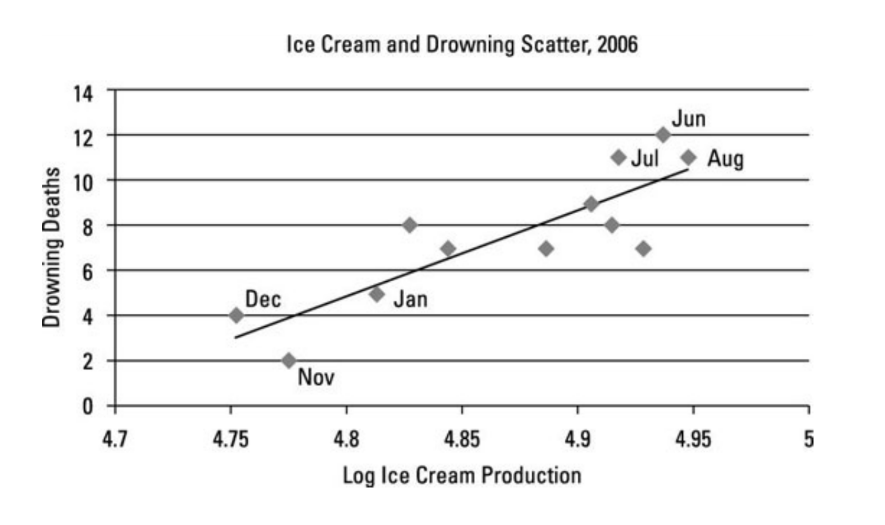
\includegraphics[width=0.7\textwidth]{img/hidden_con.png}
    \end{figure}
    \small{Does ice cream consumption cause drowning? Does the number of drownings cause ice cream cravings from the population?}
    
    \pause
    Of course not, but there is a \textbf{third variable} that causes both: the month of the year. 
\end{frame}
%%%%%%%%%%%%%%%%%%%%%%%%%%%%%%%%%%%%%%%%%%%%%%%%%%%%%%%%%%%%%%%%%%%%%%%%%%%%%%%%%%%%%%%%%%%%%%%%%%%%%%%%%%%%%%%%%%%%%%%%%
\subsection{Interventions}
%%%%%%%%%%%%%%%%%%%%%%%%%%%%%%%%%%%%%%%%%%%%%%%%%%%%%%%%%%%%%%%%%%%%%%%%%%%%%%%%%%%%%%%%%%%%%%%%%%%%%%%%%%%%%%%%%%%%%%%%%
\begin{frame}{Interventions}
    \begin{figure}[t]
        \centering
        \vspace{0pt}
        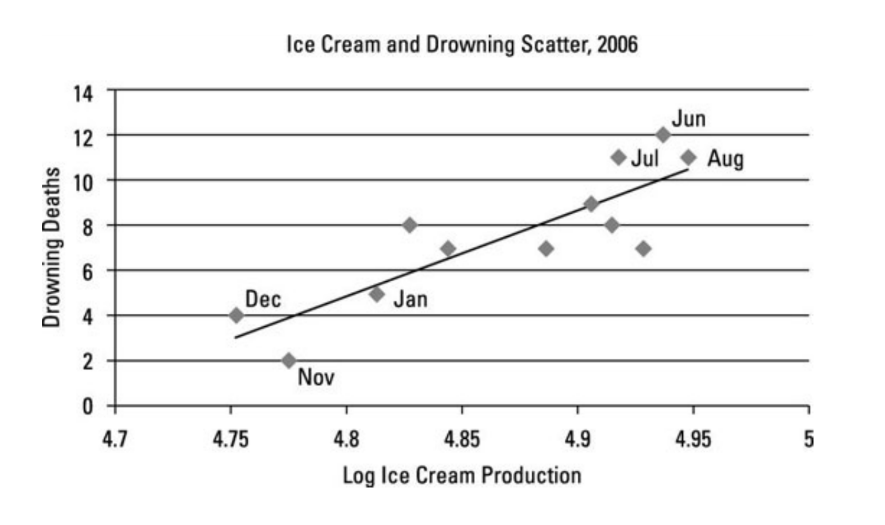
\includegraphics[width=0.7\textwidth]{img/hidden_con.png}
    \end{figure}
    But how can we know if two correlated events have a cause-effect structure? 
    \pause

    By using \textbf{interventions!}

    (e.g. If we force people to randomly eat ice cream, we will see that the number of drownings stays the same.)
\end{frame}
    

\section{Causal Reinforcement Learning}
%%%%%%%%%%%%%%%%%%%%%%%%%%%%%%%%%%%%%%%%%%%%%%%%%%%%%%%%%%%%%%%%%%%%%%%%%%%%%%%%%%%%%%%%%%%%%%%%%%%%%%%%%%%%%%%%%%%%%%%%%
\subsection{Synergies}
%%%%%%%%%%%%%%%%%%%%%%%%%%%%%%%%%%%%%%%%%%%%%%%%%%%%%%%%%%%%%%%%%%%%%%%%%%%%%%%%%%%%%%%%%%%%%%%%%%%%%%%%%%%%%%%%%%%%%%%%%

\begin{frame}{Synergies}
    \begin{itemize}
        \item \textbf{Reinforcement Learning}: Learning to achieve a goal with interventions.
        \item \textbf{Causal Learning}: Learning how the world works with interventions.
    \end{itemize}

    \pause
    \vspace{1cm}
    It looks like both of these learning methodologies revolve around \textbf{interventional data}.

    Additionally, learning a more descriptive representation of the world (through causal learning) can help
    Reinforcement Learning.
\end{frame}
%%%%%%%%%%%%%%%%%%%%%%%%%%%%%%%%%%%%%%%%%%%%%%%%%%%%%%%%%%%%%%%%%%%%%%%%%%%%%%%%%%%%%%%%%%%%%%%%%%%%%%%%%%%%%%%%%%%%%%%%%
\subsection{The Field}
%%%%%%%%%%%%%%%%%%%%%%%%%%%%%%%%%%%%%%%%%%%%%%%%%%%%%%%%%%%%%%%%%%%%%%%%%%%%%%%%%%%%%%%%%%%%%%%%%%%%%%%%%%%%%%%%%%%%%%%%%

\begin{frame}{The Field}
    The idea of joining Causality with Reinforcement Learning 
    is called recently began to be explored and is called \textbf{Causal Reinforcement Learning}.

    \begin{figure}[l]
        \centering
        \vspace{0pt}
        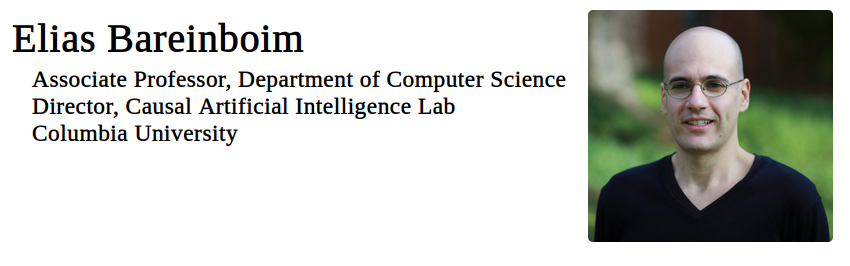
\includegraphics[width=0.7\textwidth]{img/elias.png}
    \end{figure}

    \footnotetext[3]{Source: \url{https://causalai.net/}}

\end{frame}


\section{Conclusion}
\begin{frame}{Conclusion}
    \begin{itemize}
        \item \textbf{What?}: \ding{51}
        \item \textbf{Why?}: \ding{51}
        \item \textbf{How?}: \ding{55}
        \item \textbf{Where?}: \ding{55}
    \end{itemize}
    \vspace{1cm}
    I'm still working on the \textbf{How} and \textbf{Where} parts, which correspond to the 
    \textbf{implementation} and \textbf{robotics use case}, respectively.
\end{frame}




%%%%%%%%%%%%%%%%%%%%%%%%%%%%%%%%%%%%%%%%%%%%%%%%%%%%%%%%%%%

\end{document}


